\documentclass{standalone}
\usepackage{tikz}
\usetikzlibrary{patterns, positioning}


\begin{document}
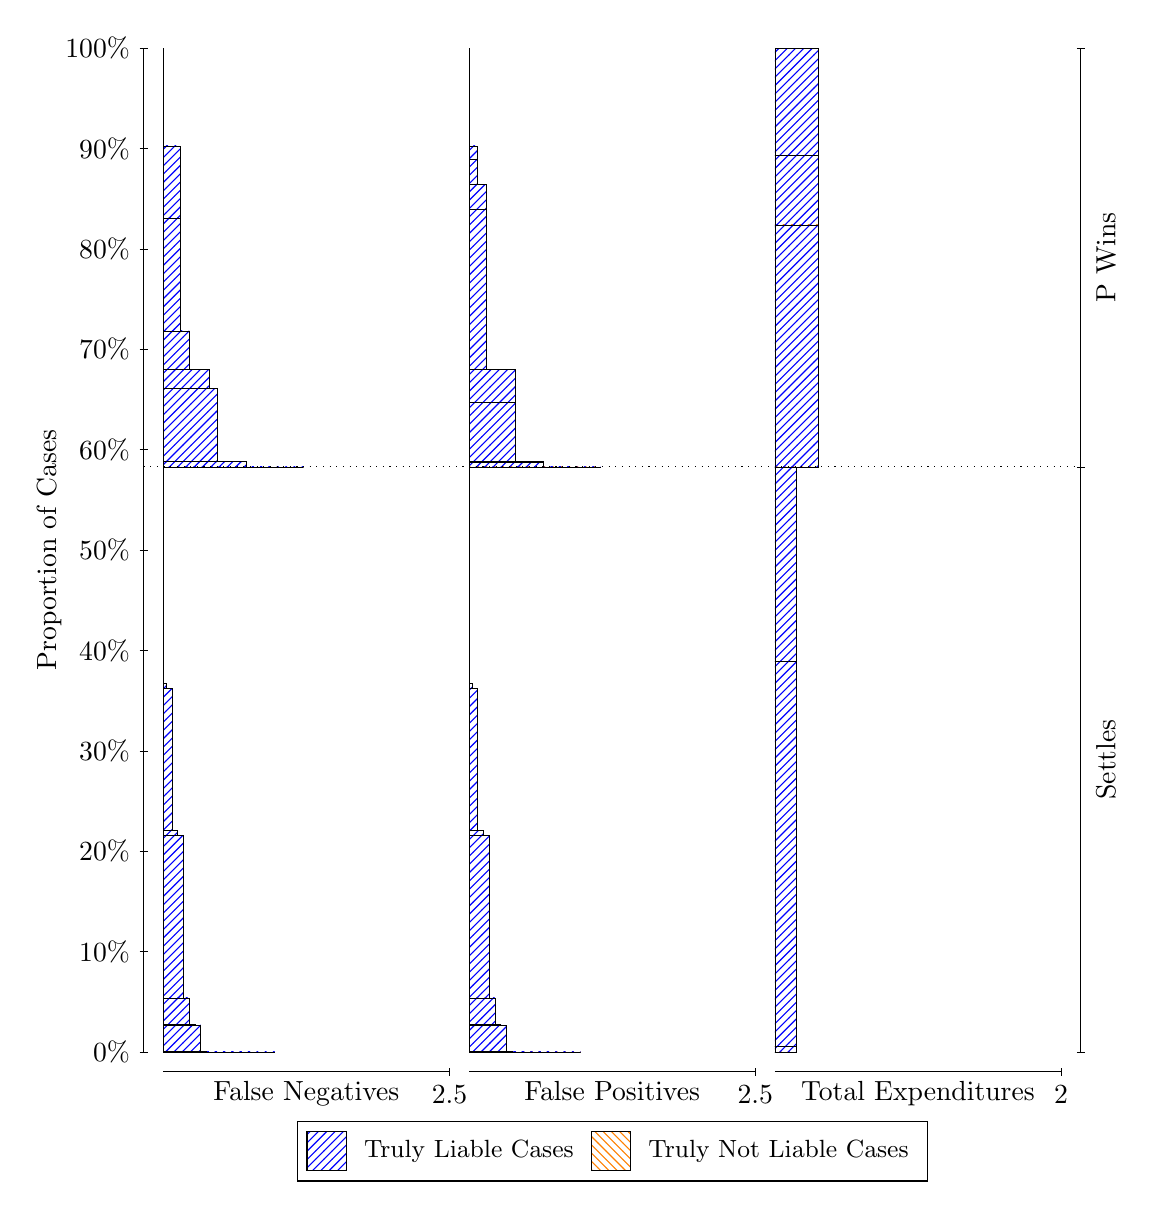
\begin{tikzpicture}
\draw[black, very thin] (1.5,1.75) -- (1.5,14.5);
\node[rotate=90, text=black, anchor=center] at (0.3, 8.125) {Proportion of Cases};
\draw[black, very thin] (1.45,1.75) -- (1.55,1.75);
\node[text=black, anchor=east] at (1.45, 1.75) {0\%};
\draw[black, very thin] (1.45,3.025) -- (1.55,3.025);
\node[text=black, anchor=east] at (1.45, 3.025) {10\%};
\draw[black, very thin] (1.45,4.3) -- (1.55,4.3);
\node[text=black, anchor=east] at (1.45, 4.3) {20\%};
\draw[black, very thin] (1.45,5.575) -- (1.55,5.575);
\node[text=black, anchor=east] at (1.45, 5.575) {30\%};
\draw[black, very thin] (1.45,6.85) -- (1.55,6.85);
\node[text=black, anchor=east] at (1.45, 6.85) {40\%};
\draw[black, very thin] (1.45,8.125) -- (1.55,8.125);
\node[text=black, anchor=east] at (1.45, 8.125) {50\%};
\draw[black, very thin] (1.45,9.4) -- (1.55,9.4);
\node[text=black, anchor=east] at (1.45, 9.4) {60\%};
\draw[black, very thin] (1.45,10.675) -- (1.55,10.675);
\node[text=black, anchor=east] at (1.45, 10.675) {70\%};
\draw[black, very thin] (1.45,11.95) -- (1.55,11.95);
\node[text=black, anchor=east] at (1.45, 11.95) {80\%};
\draw[black, very thin] (1.45,13.225) -- (1.55,13.225);
\node[text=black, anchor=east] at (1.45, 13.225) {90\%};
\draw[black, very thin] (1.45,14.5) -- (1.55,14.5);
\node[text=black, anchor=east] at (1.45, 14.5) {100\%};

\draw[black, very thin] (13.4,1.75) -- (13.4,14.5);
\draw[black, very thin] (13.35,1.75) -- (13.45,1.75);
\node[anchor=west] at (13.35, 1.75) {};
\draw[black, very thin] (13.35,9.1808) -- (13.45,9.1808);
\node[anchor=west] at (13.35, 9.1808) {};
\draw[black, very thin] (13.35,14.5) -- (13.45,14.5);
\node[anchor=west] at (13.35, 14.5) {};

\draw[black, very thin, pattern color=blue, pattern=north east lines] (1.75,1.75) rectangle (3.167,1.75);
\draw[black, very thin, pattern color=blue, pattern=north east lines] (1.75,1.75) rectangle (2.8763,1.75);
\draw[black, very thin, pattern color=blue, pattern=north east lines] (1.75,1.75) rectangle (2.8037,1.75);
\draw[black, very thin, pattern color=blue, pattern=north east lines] (1.75,1.75) rectangle (2.5857,1.7508);
\draw[black, very thin, pattern color=blue, pattern=north east lines] (1.75,1.7508) rectangle (2.513,1.7508);
\draw[black, very thin, pattern color=blue, pattern=north east lines] (1.75,1.7508) rectangle (2.4403,1.7513);
\draw[black, very thin, pattern color=blue, pattern=north east lines] (1.75,1.7513) rectangle (2.295,1.7546);
\draw[black, very thin, pattern color=blue, pattern=north east lines] (1.75,1.7546) rectangle (2.2223,2.0954);
\draw[black, very thin, pattern color=blue, pattern=north east lines] (1.75,2.0954) rectangle (2.1497,2.0983);
\draw[black, very thin, pattern color=blue, pattern=north east lines] (1.75,2.0983) rectangle (2.077,2.4361);
\draw[black, very thin, pattern color=blue, pattern=north east lines] (1.75,2.4361) rectangle (2.0043,4.5019);
\draw[black, very thin, pattern color=blue, pattern=north east lines] (1.75,4.5019) rectangle (1.9317,4.5657);
\draw[black, very thin, pattern color=blue, pattern=north east lines] (1.75,4.5657) rectangle (1.859,6.365);
\draw[black, very thin, pattern color=blue, pattern=north east lines] (1.75,6.365) rectangle (1.7863,6.4289);
\draw[black, very thin, pattern color=orange, pattern=north west lines] (1.75,6.4289) rectangle (1.75,6.4289);
\draw[black, very thin, pattern color=blue, pattern=north east lines] (1.75,6.4289) rectangle (1.75,9.1808);
\draw[black, very thin, pattern color=blue, pattern=north east lines] (1.75,9.1808) rectangle (3.5303,9.1808);
\draw[black, very thin, pattern color=blue, pattern=north east lines] (1.75,9.1808) rectangle (3.167,9.1819);
\draw[black, very thin, pattern color=blue, pattern=north east lines] (1.75,9.1819) rectangle (3.058,9.1819);
\draw[black, very thin, pattern color=blue, pattern=north east lines] (1.75,9.1819) rectangle (2.8037,9.254);
\draw[black, very thin, pattern color=blue, pattern=north east lines] (1.75,9.254) rectangle (2.6947,9.2541);
\draw[black, very thin, pattern color=blue, pattern=north east lines] (1.75,9.2541) rectangle (2.4403,10.181);
\draw[black, very thin, pattern color=blue, pattern=north east lines] (1.75,10.181) rectangle (2.3313,10.423);
\draw[black, very thin, pattern color=blue, pattern=north east lines] (1.75,10.423) rectangle (2.077,10.909);
\draw[black, very thin, pattern color=blue, pattern=north east lines] (1.75,10.909) rectangle (1.968,12.343);
\draw[black, very thin, pattern color=blue, pattern=north east lines] (1.75,12.343) rectangle (1.968,13.258);
\draw[black, very thin, pattern color=orange, pattern=north west lines] (1.75,13.258) rectangle (1.75,13.258);
\draw[black, very thin, pattern color=blue, pattern=north east lines] (1.75,13.258) rectangle (1.75,14.5);
\draw[black, very thin, pattern color=orange, pattern=north west lines] (5.6333,1.75) rectangle (7.0503,1.75);
\draw[black, very thin, pattern color=blue, pattern=north east lines] (5.6333,1.75) rectangle (7.0503,1.75);
\draw[black, very thin, pattern color=orange, pattern=north west lines] (5.6333,1.75) rectangle (6.7597,1.75);
\draw[black, very thin, pattern color=blue, pattern=north east lines] (5.6333,1.75) rectangle (6.7597,1.75);
\draw[black, very thin, pattern color=blue, pattern=north east lines] (5.6333,1.75) rectangle (6.687,1.75);
\draw[black, very thin, pattern color=orange, pattern=north west lines] (5.6333,1.75) rectangle (6.469,1.75);
\draw[black, very thin, pattern color=blue, pattern=north east lines] (5.6333,1.75) rectangle (6.469,1.7508);
\draw[black, very thin, pattern color=blue, pattern=north east lines] (5.6333,1.7508) rectangle (6.3963,1.7508);
\draw[black, very thin, pattern color=blue, pattern=north east lines] (5.6333,1.7508) rectangle (6.3237,1.7513);
\draw[black, very thin, pattern color=orange, pattern=north west lines] (5.6333,1.7513) rectangle (6.1783,1.7513);
\draw[black, very thin, pattern color=blue, pattern=north east lines] (5.6333,1.7513) rectangle (6.1783,1.7546);
\draw[black, very thin, pattern color=blue, pattern=north east lines] (5.6333,1.7546) rectangle (6.1057,2.0954);
\draw[black, very thin, pattern color=blue, pattern=north east lines] (5.6333,2.0954) rectangle (6.033,2.0983);
\draw[black, very thin, pattern color=blue, pattern=north east lines] (5.6333,2.0983) rectangle (5.9603,2.4361);
\draw[black, very thin, pattern color=orange, pattern=north west lines] (5.6333,2.4361) rectangle (5.8877,2.4361);
\draw[black, very thin, pattern color=blue, pattern=north east lines] (5.6333,2.4361) rectangle (5.8877,4.502);
\draw[black, very thin, pattern color=blue, pattern=north east lines] (5.6333,4.502) rectangle (5.815,4.5658);
\draw[black, very thin, pattern color=blue, pattern=north east lines] (5.6333,4.5658) rectangle (5.7423,6.3651);
\draw[black, very thin, pattern color=blue, pattern=north east lines] (5.6333,6.3651) rectangle (5.6697,6.4289);
\draw[black, very thin, pattern color=blue, pattern=north east lines] (5.6333,6.4289) rectangle (5.6333,9.1808);
\draw[black, very thin, pattern color=orange, pattern=north west lines] (5.6333,9.1808) rectangle (7.3047,9.1808);
\draw[black, very thin, pattern color=blue, pattern=north east lines] (5.6333,9.1808) rectangle (7.3047,9.1808);
\draw[black, very thin, pattern color=orange, pattern=north west lines] (5.6333,9.1808) rectangle (6.9413,9.1808);
\draw[black, very thin, pattern color=blue, pattern=north east lines] (5.6333,9.1808) rectangle (6.9413,9.1811);
\draw[black, very thin, pattern color=blue, pattern=north east lines] (5.6333,9.1811) rectangle (6.9413,9.1819);
\draw[black, very thin, pattern color=orange, pattern=north west lines] (5.6333,9.1819) rectangle (6.578,9.1819);
\draw[black, very thin, pattern color=blue, pattern=north east lines] (5.6333,9.1819) rectangle (6.578,9.2375);
\draw[black, very thin, pattern color=blue, pattern=north east lines] (5.6333,9.2375) rectangle (6.578,9.2541);
\draw[black, very thin, pattern color=orange, pattern=north west lines] (5.6333,9.2541) rectangle (6.469,9.2541);
\draw[black, very thin, pattern color=blue, pattern=north east lines] (5.6333,9.2541) rectangle (6.469,9.2541);
\draw[black, very thin, pattern color=orange, pattern=north west lines] (5.6333,9.2541) rectangle (6.2147,9.2541);
\draw[black, very thin, pattern color=blue, pattern=north east lines] (5.6333,9.2541) rectangle (6.2147,9.9975);
\draw[black, very thin, pattern color=blue, pattern=north east lines] (5.6333,9.9975) rectangle (6.2147,10.422);
\draw[black, very thin, pattern color=orange, pattern=north west lines] (5.6333,10.422) rectangle (6.1057,10.422);
\draw[black, very thin, pattern color=blue, pattern=north east lines] (5.6333,10.422) rectangle (6.1057,10.422);
\draw[black, very thin, pattern color=blue, pattern=north east lines] (5.6333,10.422) rectangle (6.1057,10.423);
\draw[black, very thin, pattern color=blue, pattern=north east lines] (5.6333,10.423) rectangle (5.8513,12.454);
\draw[black, very thin, pattern color=blue, pattern=north east lines] (5.6333,12.454) rectangle (5.8513,12.772);
\draw[black, very thin, pattern color=blue, pattern=north east lines] (5.6333,12.772) rectangle (5.7423,12.772);
\draw[black, very thin, pattern color=orange, pattern=north west lines] (5.6333,12.772) rectangle (5.7423,12.772);
\draw[black, very thin, pattern color=blue, pattern=north east lines] (5.6333,12.772) rectangle (5.7423,13.09);
\draw[black, very thin, pattern color=blue, pattern=north east lines] (5.6333,13.09) rectangle (5.7423,13.258);
\draw[black, very thin, pattern color=blue, pattern=north east lines] (5.6333,13.258) rectangle (5.6333,14.5);
\draw[black, very thin, pattern color=orange, pattern=north west lines] (9.5167,1.75) rectangle (9.7892,1.75);
\draw[black, very thin, pattern color=blue, pattern=north east lines] (9.5167,1.75) rectangle (9.7892,1.82);
\draw[black, very thin, pattern color=orange, pattern=north west lines] (9.5167,1.82) rectangle (9.7892,1.82);
\draw[black, very thin, pattern color=blue, pattern=north east lines] (9.5167,1.82) rectangle (9.7892,6.7066);
\draw[black, very thin, pattern color=orange, pattern=north west lines] (9.5167,6.7066) rectangle (9.7892,6.7066);
\draw[black, very thin, pattern color=blue, pattern=north east lines] (9.5167,6.7066) rectangle (9.7892,9.1808);
\draw[black, very thin, pattern color=orange, pattern=north west lines] (9.5167,9.1808) rectangle (10.062,9.1808);
\draw[black, very thin, pattern color=blue, pattern=north east lines] (9.5167,9.1808) rectangle (10.062,12.253);
\draw[black, very thin, pattern color=orange, pattern=north west lines] (9.5167,12.253) rectangle (10.062,12.253);
\draw[black, very thin, pattern color=blue, pattern=north east lines] (9.5167,12.253) rectangle (10.062,13.133);
\draw[black, very thin, pattern color=orange, pattern=north west lines] (9.5167,13.133) rectangle (10.062,13.133);
\draw[black, very thin, pattern color=blue, pattern=north east lines] (9.5167,13.133) rectangle (10.062,14.5);
\draw[black, dotted] (1.5,9.1808) -- (13.4,9.1808);
\draw[black, very thin] (1.75,1.5) -- (5.3833,1.5);
\node[text=black, anchor=north] at (3.5667, 1.5) {False Negatives};
\draw[black, very thin] (5.3833,1.45) -- (5.3833,1.55);
\node[text=black, anchor=north] at (5.3833, 1.45) {2.5};

\draw[black, very thin] (5.6333,1.5) -- (9.2667,1.5);
\node[text=black, anchor=north] at (7.45, 1.5) {False Positives};
\draw[black, very thin] (9.2667,1.45) -- (9.2667,1.55);
\node[text=black, anchor=north] at (9.2667, 1.45) {2.5};

\draw[black, very thin] (9.5167,1.5) -- (13.15,1.5);
\node[text=black, anchor=north] at (11.333, 1.5) {Total Expenditures};
\draw[black, very thin] (13.15,1.45) -- (13.15,1.55);
\node[text=black, anchor=north] at (13.15, 1.45) {2};

\node[text=black, centered, rotate=90] at (13.72, 5.4654) {Settles};
\node[text=black, centered, rotate=90] at (13.72, 11.84) {P Wins};

\draw (7.449999999999999,1.5) node[draw=none] (baseCoordinate) {};
\begin{scope}[align=center]
        \matrix[scale=0.5, draw=black, below=0.5cm of baseCoordinate, nodes={draw}, column sep=0.1cm]{
            \node[rectangle, draw, minimum width=0.5cm, minimum height=0.5cm, pattern color=blue, pattern=north east lines] {}; &
            \node[draw=none, font=\small, text=black] (B) {Truly Liable Cases}; &
            \node[rectangle, draw, minimum width=0.5cm, minimum height=0.5cm, pattern color=orange, pattern=north west lines] {}; &
            \node[draw=none, font=\small, text=black] (B) {Truly Not Liable Cases}; \\
            };
\end{scope}

\end{tikzpicture}
\end{document}